\documentclass{standalone}
\usepackage{tikz}   %TikZ is required for this to work.  Make sure this exists before the next line
\usetikzlibrary{arrows.meta}

\begin{document}
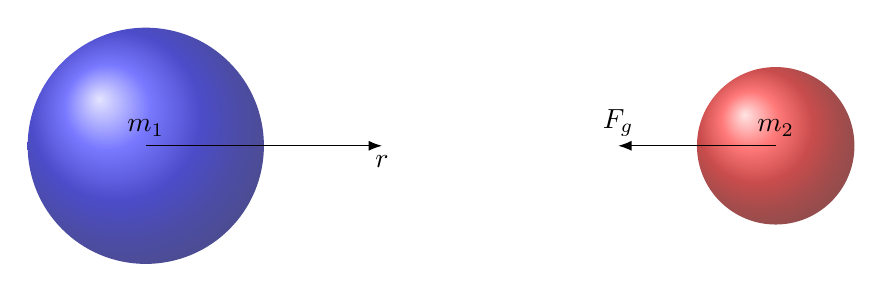
\begin{tikzpicture}
    \coordinate (m1) at (0, 0);
    \coordinate (m2) at (8, 0);

    \shade[ball color=blue, opacity=0.7] (m1) circle (1.5);
    \shade[ball color=red, opacity=0.7] (m2) circle (1);

    \node[ above] at (m1) {$m_1$};
    \node[above] at (m2) {$m_2$};

    \draw[-Latex] (m1) -- ++(3, 0) node[below ] {$r$}; 
    \draw[-Latex] (m2) -- ++(-2, 0) node[above] {$F_g$};
\end{tikzpicture}
\end{document}
